In this section, we show the optimization details done through this work. We discuss the statistics of the new database and the schema changes. Moreover, other optimization techniques related to query, indexes and memory are discussed, as well.

\subsection{New Database Statistics}
In this subsection, we show the new database statistics after optimization. The record count is extracted from the database filled with $100000$ records per table. Other filling sizes are considered through the analysis like $10000$ and $1000000$. \\

\begin{tabular}{||c | c | c | c | c||} 
 \hline
 Table Name & Row Count & Main Key & Indexes & FK  \\ [0.5ex] 
 \hline\hline
 Disaster & 100000 & YES & 4 & 2 \\ 
 \hline\hline
 Causes & 100000 & YES & 1 & 1 \\ 
 \hline\hline
 Precautions & 100000 & YES & 1 & 1 \\ 
 \hline\hline
 Incident & 100000 & YES & 4 & 3 \\ 
 \hline\hline
 Descriptions & 100000 & YES & 1 & 1 \\ 
 \hline\hline
 Casualty & 25000 & YES & 1 & 0 \\ 
 \hline
 Government\_Representative & 25000 & YES & 1 & 0 \\
 \hline
 Govn\_Rep\_Credentials & 25000 & YES & 1 & 1 \\
 \hline
 Citizen & 25000 & YES & 1 & 0 \\
 \hline
 Citizen\_Credentials & 25000 & YES & 1 & 1 \\
 \hline
 Criminal & 25000 & YES & 1 & 0 \\
 \hline
 Report & 100000 & YES & 5 & 4 \\
 \hline
 Report\_Content & 100000 & YES & 1 & 1 \\
 \hline
 Casualty\_Incident & 100000 & YES \emph{(Composite)} & 3 & 2 \\ [1ex] 
 \hline
\end{tabular} \\

\begin{tabular}{||c | c | c||} 
 \hline
 Table Name & Identity Column & Max Row Size (Bytes) \\ [0.5ex] 
 \hline\hline
 Disaster & YES & 52 \\ 
 \hline
 Causes & YES & 65538 \\ 
 \hline
 Precautions & YES & 65538 \\ 
 \hline
 Incident & YES & 120 \\ 
 \hline
 Descriptions & YES & 65538 \\ 
 \hline
 Casualty & YES & 105 \\ 
 \hline
 Government\_Representative & YES & 116 \\ 
 \hline
 Govn\_Rep\_Credentials & YES & 103 \\ 
 \hline
 Citizen & YES & 116 \\ 
 \hline
 Citizen\_Credentials & YES & 103 \\ 
 \hline
 Criminal & YES & 106 \\ 
 \hline
 Report & YES & 23 \\ 
 \hline
 Report\_Content & YES & 65538 \\ 
 \hline
 Casualty\_Incident & NO & 6 \\ [1ex] 
 \hline
\end{tabular}

\subsection{Schema Optimization}
The following database schema shows the optimizations over the old schema. The schema optimizations can be summarized as follows :
\begin{enumerate}
    \item \textbf{Denormalization} of \emph{Person} table with all persons types. This is mainly because no duplicates between persons types. For example, no person can be a casualty and a criminal at the same time. So, in order to avoid redundant joins, the \emph{Person} relation is merged into the four child relations.
    \item \textbf{Normalization} \emph{(Vertical Partitioning)} of variable-size data. The access of fixed-size records is faster than that of variable-size data, as the \emph{DBMS} don't require to pre-calculate the record size. That's why, the variable-size data like \emph{text}, \emph{usernames} and \emph{passwords} are separated into separate relations. One more reason for doing so is that the data in these fields aren't accessed frequently, so they better be separate from other frequently-accessed data.
    \item \textbf{Minimization} of the data types based on semantic and statistical \emph{heuristics}. The data types of different fields are reduced to the minimum possible size, in order to ease their read and write to the disk. For example, all \emph{primary keys} are reduced to \texttt{MEDIUMINT}, because the table size is at most $1000000$. Moreover, Some fields that are just limited to range from $1$ to $10$ are reduced to $4$ bits instead of \texttt{INT}.
    \item \textbf{Conversion} of variable-size data to fixed-size data. As the fixed-size record are faster to access and transfer, so each \emph{VarChar} is converted into \emph{Char}. This, however, can increase the storage space, as \emph{Char} allocates the target bytes whatever they are all used or not.
    \item \textbf{Usage} of \texttt{NOT NULL}, whenever possible. If the field isn't marked as \texttt{NOT NULL}, it allocates extra bits to check whether the field is \emph{NULL} or not.
\end{enumerate}
\begin{figure}[H]
    \centering
    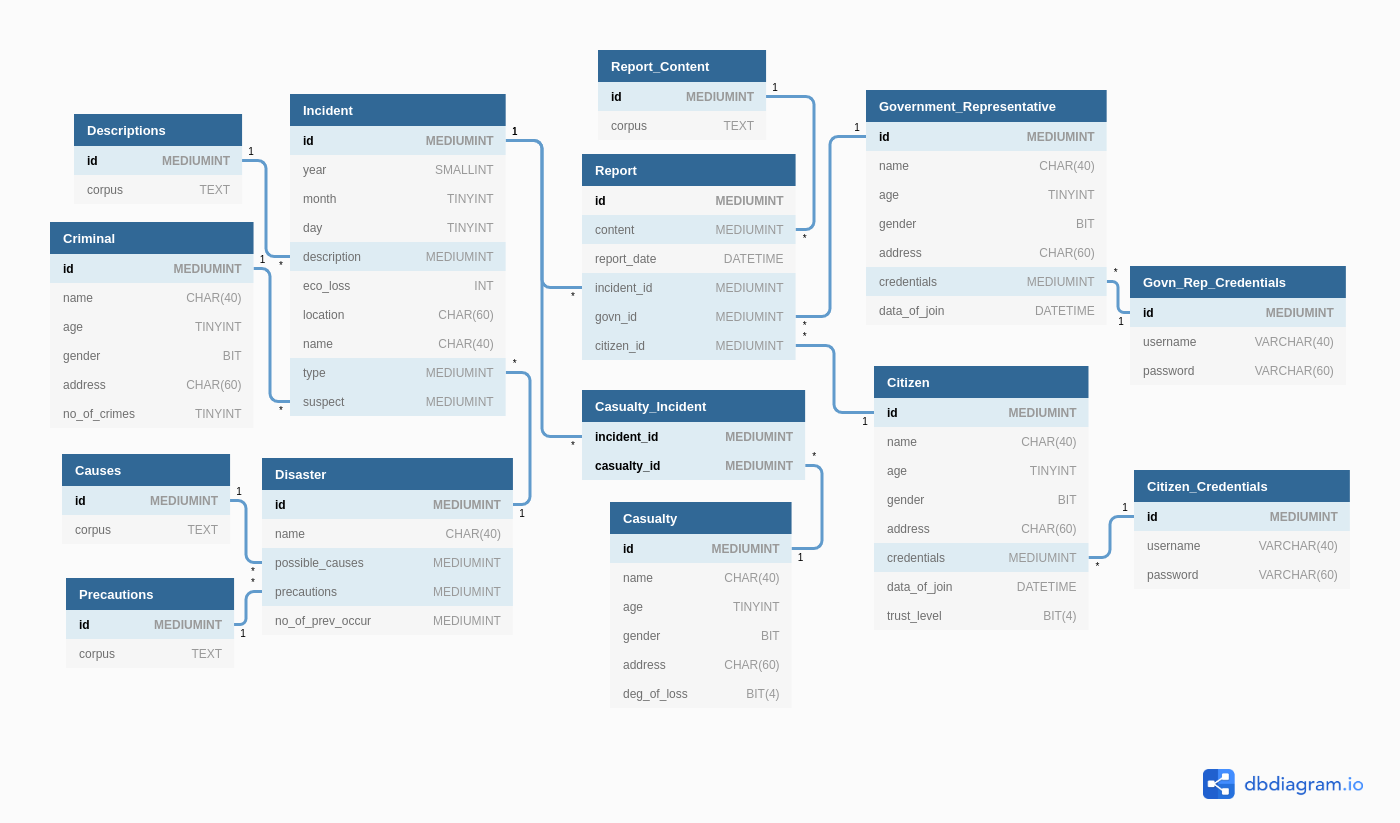
\includegraphics[width=\textwidth]{images/stats/optimized-schema.png}
    \caption{New Optimized Database Schema.}
    \label{fig:db-schema}
\end{figure}

\subsection{Memory Optimization}
In \emph{MySQL}, the memory optimization can be done through changing the memory system variables of the \emph{DBMS} given the same hardware. The system variables can include \texttt{innodb\_buffer\_pool\_size}, \texttt{innodb\_buffer\_pool\_chunk\_size} and \emph{innodb\_buffer\_pool\_instances}. We can, also, switch between the two storage engines of \emph{MySQL}, which are \texttt{INNODB} and \texttt{MyISAM}. \\

We tried both storage engines and discovered that using \texttt{INNODB} gives much better performance based on our database schema. Moreover, we tried to optimize most of the system variables, however some changes are \textbf{prohibited} by \emph{MySQL} and other changes don't affect the performance at all. The only change that results in significant improvement is increasing \texttt{innodb\_buffer\_pool\_size}. \\

So, we can summarize our \emph{memory optimization} as follows :
\begin{itemize}
    \item Usage of \texttt{INNODB} as a storage engine, which is much faster.
    \item Increasing \texttt{INNODB}'s buffer pool size, which is responsible for the amount of memory allocated for \emph{DBMS} operations, from \emph{32MB} to \emph{4GB}.
\end{itemize}

\subsection{Index Tuning}
Using indexes on fields that are frequently used in our queries makes them much faster like creating indexes on fields that we use in search or sort, especially if these fields are strings. As shown in \textbf{\textit{Query 2}}, creating index on \textbf{Incident.name} will boost up the performance as index field is a sorted data structure that makes searching process much faster (log IO/CPU complexity rather than linear one). creating indexes on \textbf{Incident.year}, \textbf{Incident.month}, \textbf{Incident.day}, \textbf{Incident.eco\_loss} will make it further faster.

\subsection{Query Rewriting}
\subsubsection{OR performs better than UNION in IN conditions}
In \textbf{IN} conditions, using \textbf{UNION} adds overhead on checking all conditions one at a time, but in \textbf{OR}, The condition is considered true once one of the conditions is evaluated as \textbf{TRUE}.
As shown in \textbf{\textit{Query 2}}, once \textbf{Incident.year} is equal to 2010, no need to check the remaining conditions.

\subsubsection{UNION ALL is faster than UNION}
\textbf{UNION ALL} doesn't remove duplicates but \textbf{UNION} does, so whenever \textbf{UNION} and \textbf{UNION ALL} are equivalent, use \textbf{UNION ALL} as shown in \textbf{\textit{Query 2}}. For example, if we are trying to union mutually exclusive columns (no mutual information), using \textbf{UNION ALL} will be much faster.

\subsection{Semantic and Statistic Query Optimization}
Remove constraints specified on the database which are semantically or statistically guaranteed to happen, as it adds unneeded overhead without any use.
\subsubsection{Semantic Constraints}
Constraints that are guaranteed to happen based on the physical meaning of the database, like :
\begin{itemize}
     \item Our database includes a gender field that can be only males and females, so no need to specify that :
     \begin{verbatim}
     Person.gender IN (0,1)
     \end{verbatim}
     \item If we need to retrieve all not recent Incidents that happened before 5 years at least and are reviewed by not recent government representatives that started their job before 5 years at least, no need to mention both, as for sure if an incident happened say 6 years ago, it's guaranteed that its government representative reviewed it 6 years ago, so it's guaranteed that he/she is not recent as well.
     Use :
     \begin{verbatim}
     Incident.year > 5
     \end{verbatim}
     Instead of:
     \begin{verbatim}
     YEAR(Government_Representative.date_of_join) > 5 
     and Incident.year > 5
     \end{verbatim}
\end{itemize}

\subsubsection{Statistic Constraints}
Constraints that are guaranteed to happen based on the current statistics of the database, like:
\begin{itemize}
     \item All Government Representatives are older than 20 years old in the database statistics, so no need for :
     \begin{verbatim}
     Government_Representative.age >= 20
     \end{verbatim}
     \item All Citizens have trust level up to 10 in the database statistics, so no need for :
     \begin{verbatim}
     Citizen.trust_level <= 10
     \end{verbatim}
\end{itemize}

\subsection{Used Optimizations in our Queries}
\subsubsection{Query 1}
\begin{itemize}
    \item  Schema Optimization.
    \item  Memory Optimization.
    \item  Semantic and Statistic Query Optimization.
\end{itemize}

\subsubsection{Query 2}
\begin{itemize}
    \item  Schema Optimization.
    \item  Memory Optimization.
    \item  Index Tuning.
    \item  Query Rewriting -  OR performs better than UNION in IN conditions.
    \item  Query Rewriting - UNION ALL is faster than UNION.
\end{itemize}

\subsubsection{Query 3}
\begin{itemize}
    \item  Schema Optimization.
    \item  Memory Optimization.
    \item  Index Tuning.
    \item  Query Rewriting.
\end{itemize}

\subsubsection{Query 4}
\begin{itemize}
    \item  Schema Optimization.
    \item  Memory Optimization.
\end{itemize}

\subsubsection{Query 5}
\begin{itemize}
    \item  Schema Optimization.
    \item  Memory Optimization.
    \item  Semantic and Statistic Query Optimization.
\end{itemize}
